%\begin{center}
%\rule[0pt]{\textwidth}{1pt}\\[7pt]
%{\LARGE {This chapter is due}}
%\rule[0pt]{\textwidth}{1pt}
%\end{center}
\section{Approximate \SVP on a $q$-ary lattice} 
\label{sec:ApproxQary}

In this section we present a combinatorial algorithm that solves the approximate shortest vector problem, $\appSVP$, on a $q$-ary lattice. As opposed to the algorithm from the previous section where the approximation factor $\gamma$ was a constant, here $\gamma$ is polynomial in the lattice-dimension, i.e.\ we look for a vector $\vvec$ from $\qLat \subset \Z_q^n$ s.t.\ $\| \vvec \| \leq \poly(n) \lambda_1(\qLat)$.

An algorithm for $\appSVP$ with a polynomial approximation factor gives a way to solve the so-called Short Integer Solution Problem (\SIS) -- the problem introduced by Ajtai in \cite{STOC:Ajtai96} that serves as the foundation for a variety of cryptographic primitives. Given a matrix $\AMat \in \Z_q^{n \times m}$ composed column-wise from uniformly chosen $\avec_i \in \Z_q^n$, \SIS asks to find a short $\vvec \in \Z_q^m$ s.t.\ $\AMat \vvec = 0 \mod q$. The length condition is specified by an input parameter $\beta$, i.e. the output $\vvec$ must satisfy $\| \vvec \| \leq \beta$, where $ \beta=\poly(n)$ and the degree of the polynomial depends on the modulus $q$. Note that we are not interested in the trivial solution $\vvec = (q, 0, \ldots, 0)$. Also notice that if we ask for $\vvec \in \ZO{n}$, \SIS becomes the vectorial Subset Sum Problem.

To see the connection between \SIS and the approximate \SVP, let us consider an $m$-dimensional $q$-ary lattice $\qLATTp(\AMat) = \{ \xvec \in \Z^m \colon \AMat \xvec = 0 \mod q \}$. A solution to $\appSVP$ on $\qLATTp(\AMat)$ is a vector $\vvec \in \qLATTp(\AMat)$ of length $\|\vvec \| \leq \gamma \lambda_1(\qLATTp(\AMat))$ and therefore, it is a solution to the \SIS problem when $\gamma$ is appropriately chosen. From Minkowski's bound we know that $\lambda_1(\qLATTp(\AMat) \leq \sqrt{m} q^{n/m}$. Hence, if we set $q=\bigO(n^{\cq})$ (as we did in Chap.~\ref{chap:LWEasBDD} for the analysis of \LWE), $\gamma  = \bigO(n^{\cg})$ for constants $\cq>1, \cg$, and take $m = \TLandau(n)$, a solution for $\appSVP$ will be a vector of length $\|\vvec \| \leq n^{\cg + \cq/2 + 1/2}$. Values of $\cg$ stem from the connection of \SIS to the worst-case lattice-problems. Since Ajtai's proof, the constant has been improved from the original $\cg=8+\smallo(1)$ \cite{STOC:Ajtai96} down to $\cg=2.5+\smallo(1)$ in \cite{Mic05} and, finally, to $\cg=1+\smallo(1)$ in \cite{FOCS:MicReg04}. In the language of \SIS, $\cg$ is known as Ajtai's connection factor.

We have a natural restriction on $\cg$ that comes from the fact that we want to avoid trivial solutions of length $q$, namely $\cg<\cq/2 - 1/2$. 

Notice that we already mentioned $\appSVP$ in Sect.~\ref{sec:OtherAttacks} when we discussed the so-called $\Dual$ attack on \LWE. The name of the attack comes from the fact that the two problems, \LWE and \SIS, are `dual' to each other. What it means is that the \LWE problem -- the decoding problem on $\Lat(\AMat\transpose)$ -- can be solved using a \SIS oracle for $\AMat$ (or, equivalently, an oracle for $\appSVP$ on $\qLATTp(\AMat)$) as we have already seen in Alg.~\ref{alg:Dual}, Chap.~\ref{chap:LWEasBDD}. The two lattices, $\Lat(\AMat\transpose)$ and $\qLATTp(\AMat)$, are dual to each other up to scaling by $q$: $\qLat(\AMat\transpose)^* = \frac{1}{q} \qLATTp(A)$, $\qLATTp(A)^* = \frac{1}{q}\qLat(\AMat\transpose)$.  
We refer the reader to \cite{Mic10} for more interesting outcomes of this duality.

In the following sections we present two combinatorial algorithms for $\appSVP$ on $\qLATTp(\AMat)$ in case $\gamma =\poly(n)$. The second algorithm has a better constant in the running time exponent. Next, we compare our algorithms with the \BKZ reduction run on $\qLATTp(\AMat)$ when the block-size $\beta$ is chosen s.t.\ the first vector of the reduced basis is a solution to $\appSVP$. We conclude that our improved algorithm outperforms \BKZ for some values of $\cq, \cg$ even when $\BKZ$ is instantiated with the best known heuristic \SVP oracle.


\subsection{An algorithm for $\appSVP$ on a $q$-ary lattice} \label{subsec:qAryAlg}

In this section, we present a combinatorial algorithm that on input $\AMat \in \Z_q^{n \times 2n}$ and $\cg < \cq/2 - 1/2$, outputs a vector $\vvec \in \qLATTp(A) \subset \Z_q^{2n}$ s.t.\ $\| \vvec \| \leq n^{\cg+\cq/2+1/2}$. Notice that we set the lattice dimension $m$ as $m=2n$. This choice simplifies the exposition and is necessary for the improved algorithm described in Sect.~\ref{subsec:qAryAlgImproved}. Case $m=\cm n$ for $\cm = \TLandau(1)$ is considered in Rmk.~\ref{rmk:Linm}.%We make such a choice of $m$ for two reasons. First, it simplifies the description of the algorithms and, second, another constant will not make our algorithm faster. 

The algorithm is actually a combinatorial \BKW-type algorithm for \LWE due to Kirchner-Fouque \cite{C:KirFou15} and Guo et al.\ \cite{C:GuoJohSta15} adapted to the $\appSVP$ problem. We now give its high-level overview.

The idea is to split the dimension of the lattice, $2n$, into $k$ blocks $d_1, \ldots, d_k$, i.e.\ $\sum_{i=1}^k d_i = 2n$. We also choose $k$  positive values $R_1, \ldots, R_k$ where $R_i < q/2$ for all $i$. The algorithm proceeds in $k$ steps. 

On Step 1, we search for pairs of lattice-vectors $(\vvec_1, \vvec_2)$ s.t.\
\[
\Big\lfloor \frac{[\vvec_1]_1^{d_1}}{R_1} \Big\rceil =  \Big\lfloor \frac{[\vvec_2]_1^{d_1}}{R_1} \Big\rceil\footnote{Recall the notation $[\xvec]_i^j = x_i\ldots x_j$ for $i \leq j$.}.
\]
In other words, we split our $q$-ary cube $[-\frac{q-1}{2}, \frac{q-1}{2}]^{d_1}$ (assume $q$ is odd, the algorithm can be easily adapted for an even $q$) into many smaller cubes $[-R_1, R_1]^{d_1}$ and search for pairs $(\vvec_1, \vvec_2)$ that on their first $d_1$ coordinates lie in the same cube. In our algorithm we set $R_1 = n^{\smallo(1)} \ll q $, and we can adjust our choice for $R_1$ s.t. the small cubes split the large cube evenly. See Fig.~\ref{fig:Bucketing} for a $2$-dimensional example. 

Once two such vectors are found, we subtract one from the other and put the result into list $L_1$. Important is that we can bound the $\ell_{\infty}$-norm of elements in $L_1$: on average, $\| [\vvec_1 - \vvec_2]_1^{\d_1}\|_{\infty} \leq \sqrt{2}R_1$. The output of Step 1 are many vectors with \emph{bounded} $\ell_{\infty}$-norm on their first $d_1$ coordinates. On Step 2, we use vectors from $L_1$ to search for pairs that lie in the same $[-R_2, R_2]^{\d_2}$ cube on their $d_1+1, \ldots, d_2$ coordinates analogously to Step 1. The output of Step 2 is a list $L_2$ with vectors bounded in $\ell_{\infty}$-norm on coordinates $1, \ldots, d_1$ and $d_1+1, \ldots, d_2$.  

Repeating this procedure for all $k$ steps, we end up with lattice-vectors for which we can bound their $\ell_{\infty}$-norm on all the $2n$ coordinates and hence, their Euclidean norm. From the upper-bound on the length of the output, we find an optimal on $k$. We defer the discussion on how to set $R_i$'s and $k$ to the next section. 

\begin{figure}[t]
	\centering
	\begin{tikzpicture}
	\draw[gray!20, ->] (-90pt,0) -- (90pt,0);
	\draw[gray!20, ->] (0,-80pt) -- (0,80pt);
	
	 \draw[thick] (-60pt, -60pt) rectangle (60pt, 60pt);
	 \draw (-60pt, 0)  node[below left] {\scriptsize $-\tfrac{q-1}{2}$};
	 \draw (60pt, 0)  node[below right] {\scriptsize $\tfrac{q-1}{2}$};
	 
	 \draw[very thin] (-20pt, -60pt) -- (-20pt, 60pt);
	 \draw[very thin] (20pt, -60pt) -- (20pt, 60pt);
	 \draw[very thin] (-60pt, -20pt) -- (60pt, -20pt);
	 \draw[very thin] (-60pt, 20pt) -- (60pt, 20pt);
	 
	 \draw [decoration={brace, mirror, raise=7pt},
	 		decorate,below=10pt, yshift=5pt](-20pt, 0) -- (20pt, 0) node [black,midway, yshift=-8pt] {\scriptsize $R$};
	 		
	 \filldraw (45pt, 45pt) circle (1pt) node[below right, xshift=-3pt, yshift=2pt] {\tiny $\vvec_1$};
	 \filldraw (32pt, 35pt) circle (1pt) node[below left, xshift=6pt, yshift=2pt] {\tiny $\vvec_2$};
	 
	 \draw [decoration={brace, raise=5pt},
	 	 		decorate,above=10pt, yshift=-3pt, xshift=2pt](32pt, 35pt) -- (45pt, 45pt) node [black,midway, rotate=37, yshift=5pt, xshift=-4pt] {\tiny $ \leq \mkern-6mu \sqrt{2}R$};
	 	 		
	%----------LABELS---------
	\node[draw=none] at (10pt, -15pt){\tiny $(0,0)$};
	\node[draw=none] at (10pt, 25pt){\tiny $(0,1)$};	
	\node[draw=none] at (10pt, -55pt){\tiny $(0,-1)$};
	
	\node[draw=none] at (50pt, 25pt){\tiny $(1,1)$};
	\node[draw=none] at (50pt, -15pt){\tiny $(1,0)$};
	\node[draw=none] at (50pt, -55pt){\tiny $(1,-1)$};
	
	\node[draw=none] at (-30pt, 25pt){\tiny $(1,-1)$};
	\node[draw=none] at (-30pt, -15pt){\tiny $(-1,0)$};
	\node[draw=none] at (-33pt, -55pt){\tiny $(-1,-1)$};
	\end{tikzpicture}
	\caption[Bucketing on a $2$-dimensional $q$-ary lattice]{Bucketing on a $2$-dimensional $q$-ary lattice. Each small cube of length $R$ gets its two-dimensional label. The vectors $\vvec_1$, $\vvec_2$ appear in the same bucket $(1, 1)$ and, hence, the $\ell_2$-norm of their difference is bounded by $\sqrt{2}R$.}
	\label{fig:Bucketing}
\end{figure}

There is one simple trick which greatly improves the running time of the algorithm. We can write our input matrix $\AMat \in \Z_q^{n \times 2n}$ as $\AMat = [\AMat_1 | \AMat_2]$ where $\AMat_i \in \Z_q^{n \times n}$. With high probability, we have that $\AMat_1$ is invertible $\bmod~q$ allowing us to write $\AMat = [\Id_n | \AMat']$ where $\AMat' = \AMat_1^{-1} \AMat_2 \bmod q$. Essentially this procedure brings a $q$-ary code generated by $\AMat$ to a systematic form. It is easy to verify that a basis for $\qLATTp(\AMat)$ is of the form (cf. with the basis $B$ for $\qLat(\AMat\transpose)$ given in Eq.~(\ref{eq:LWEBasis})):
\begin{equation}\label{eq:BasisD}
	\DMat = \begin{pmatrix}
	-\AMat' & q\Id_n \\
	\Id_{n} & 0
	\end{pmatrix}.
\end{equation}


\begin{algorithm}[t]
	\caption{$\appSVP$ on a $q$-ary lattice}
	\label{alg:ApproxSVP}
	\textbf{Input:} $D$ -- a basis for the lattice $\qLATTp(A) \subset \Z_q^{2n}$ defined as in Eq.~(\ref{eq:BasisD}), $\gamma = n^{\cg}$ -- the approximation factor, $\cg>0$ \\
	\textbf{Output:} $L_k$ -- list of vectors from $\qLATTp(A)$ with vectors of norm $\| \vvec \| \leq n^{\cg+\cq/2+1/2}$;
	
	\begin{algorithmic}[1]
		
		\State Set the sieving bounds $R_i$ as $R_1 = n^{\smallo(1)}$ and $R_i = \sqrt{2}^{i-1} R_1$ for $i \geq 2$.
		\State Set the lengths of blocks $d_i$ as in Eq.~(\ref{eq:d_i}) and the boundaries of each block $(l_{i-1}, \ldots, l_i)$ s.t.\ $l_{i}-{l_{i-1}} = d_i$ and $l_k = 1, l_0 = n$.
		
		\Repeat \Comment{Create the list $L_0$}
		\State Choose $\xvec \in \Z_q^{2n}$ s.t.\ $\| [\xvec]_{n+1}^{2n} \|_{\infty} \leq R_1$
		\State $L_0 \gets L_0 \union \{D\xvec \bmod q\} $
		\Until{$L_0$ is large enough}
		
		\State $T \gets \emptyset$ \Comment{Initialize an array $T$ indexed by buckets}
		\ForAll {$i=1 \ldots k$} \label{algline:ForLoop1}
			\ForAll { $\vvec \in L_{i-1}$} \label{algline:ForLoop2}
				\State $b \gets \Big\lfloor \frac{[\vvec]_{l_i}^{l_{i-1}}}{R_i} \Big\rceil$ \Comment Find the bucket for $\vvec\mkern2mu[l_i, \ldots, l_{i-1}]$
				\If{$T[b] = \emptyset$}
					\State $T[b] \gets \vvec$
				\Else
					\State $L_{i} \gets L_{i} \union \{T[b] - \vvec \}$
					\State $T[b] \gets \emptyset$
				\EndIf
			\EndFor
		\EndFor
		\State \Return $L_k$
	\end{algorithmic}
	
	\vspace{10pt}
	
\end{algorithm}

\begin{figure}[H]
	\centering
	\begin{tikzpicture}[]
	\tikzset{
		List/.style={
			rectangle split, rectangle split horizontal,  
			draw=black, thick,
			%text width=10em,
			inner sep=6pt,
		} 
	}    
	\matrix (m) [row sep=0.8em, column sep=3em]{
		\node[](L0) {$L_0:$}; & 
		\node[List, rectangle split parts=3, name=list, rectangle split part fill={black!60,black!60,black!10}] (list) {
			\nodepart[text width=5.4cm]{one}{}
			\nodepart[text width=0.6cm]{two}
			\nodepart[text width=6cm] {three}};
		
		\draw [decoration={brace, raise=5pt},
		decorate,below=10pt] (list.two split north) -- (list.north east) node [black,midway, yshift=20pt] {\scriptsize $n$}; 
		
		\draw [decoration={brace,raise=5pt},
		decorate,below=10pt](list.one split north) -- (list.two split north) node [black,midway, yshift=20pt] {\scriptsize $d_1$};
		
		\draw [decoration={brace, mirror, raise=5pt},
		decorate,below=10pt](list.two split south) -- (list.south east) node [black,midway, yshift=-10pt] {\scriptsize $\leq R_1$};
		
		\draw [decoration={brace, mirror, raise=5pt},
		decorate,below=10pt](list.south west) -- (list.two split south) node [black,midway, yshift=-10pt] {\scriptsize $\leq q/2$};
		\draw [decoration={brace,raise=18pt},
		decorate,below=10pt](list.north west) -- (list.north east) node [black,midway,yshift=30pt] {\scriptsize $2n$};\\[-1ex]
		%---------------------------------------  
		\node[](L1) {$L_1:$}; & 
		\node[List, rectangle split parts=4, name=list2, rectangle split part fill={black!60,black!60,black!15,black!15}] (list2) {
			\nodepart[text width=4.2cm]{one}{}
			\nodepart[text width=0.8cm]{two}
			\nodepart[text width=0.6cm] {three}
			\nodepart[text width=6cm] {four}};
		
		\draw [decoration={brace,raise=5pt},
		decorate,below=10pt](list2.three split north) -- (list2.north east) node [black,midway, yshift=20pt] {\scriptsize $n$}; 
		
		\draw [decoration={brace,raise=5pt},
		decorate,below=10pt](list2.two split north) -- (list2.three split north) node [black,midway, yshift=20pt] {\scriptsize $d_1$};
				
				
		\draw [decoration={brace, mirror, raise=5pt},
		decorate,below=10pt](list2.two split south) -- (list2.south east) node [black,midway, yshift=-10pt] {\scriptsize $\leq \sqrt{2}R_1$};

		
		\draw [decoration={brace,raise=5pt},
		decorate,below=10pt](list2.one split north) -- (list2.two split north) node [black,midway, yshift=20pt] {\scriptsize $d_2$};
		
		\draw [decoration={brace, mirror, raise=5pt},
		decorate,below=10pt](list2.south west) -- (list2.two split south) node [black,midway, yshift=-10pt] {\scriptsize $\leq q/2$};\\ [-1ex]
		
		%---------------------------------------  
		\node[](L2) {$L_2:$}; & 
		\node[List, rectangle split parts=5, name=list3, rectangle split part fill={black!60,black!60,black!30,black!30,black!30}] (list3) {
					\nodepart[text width=3.0cm]{one}{}
					\nodepart[text width=0.8cm]{two}
					\nodepart[text width=0.8cm]{three}
					\nodepart[text width=0.6cm] {four}
					\nodepart[text width=6cm] {five}};
				
		\draw [decoration={brace,raise=5pt},
		decorate,below=10pt](list3.four split north) -- (list3.north east) node [black,midway, yshift=20pt] {\scriptsize $n$}; 
				
		\draw [decoration={brace,raise=5pt},
		decorate,below=10pt](list2.two split north) -- (list2.three split north) node [black,midway, yshift=20pt] {\scriptsize $d_1$};
								
		\draw [decoration={brace, mirror, raise=5pt},
		decorate,below=10pt](list3.three split south) -- (list3.south east) node [black,midway, yshift=-10pt] {\scriptsize $\leq 2 R_1$};
		
		\draw [decoration={brace,raise=5pt},
		decorate,below=10pt](list3.two split north) -- (list3.three split north) node [black,midway, yshift=20pt] {\scriptsize $d_2$};
				
		\draw [decoration={brace, mirror, raise=5pt},
		decorate,below=10pt](list3.two split south) -- (list3.three split south) node [black,midway, yshift=-10pt] {\scriptsize $\leq  \mk \sqrt{2}R_2$};
		
		\draw [decoration={brace,raise=5pt},
		decorate,below=10pt](list3.one split north) -- (list3.two split north) node [black,midway, yshift=20pt] {\scriptsize $d_3$};
		
		\draw [decoration={brace, mirror, raise=5pt},
		decorate,below=10pt](list3.south west) -- (list3.two split south) node [black,midway, yshift=-10pt] {\scriptsize $\leq q/2$};\\ [-3ex]
		
		\node[] (vd) {$\vdots$}; &
		\node[]{$\vdots$}; \\ [-3ex]
		%---------------------------------------  
		
		\node[](Lk) {$L_k:$}; & 
		\node[List, rectangle split parts=6, name=list4,rectangle split part fill={black!40,black!40,black!40,black!40,black!40,black!40}] (list4) {
			\nodepart[text width=1.8cm]{one}{}
			\nodepart[text width=0.6cm]{two}{$\ldots$}
			\nodepart[text width=0.8cm]{three}
			\nodepart[text width=0.8cm] {four}
			\nodepart[text width=0.6cm] {five}
			\nodepart[text width=6cm] {six}};
		
		\draw [decoration={brace,raise=5pt},
		decorate,below=10pt](list4.five split north) -- (list4.north east) node [black,midway, yshift=20pt] {\scriptsize $n$}; 
		
		\draw [decoration={brace,raise=5pt},
		decorate,below=10pt](list4.four split north) -- (list4.five split north) node [black,midway, yshift=20pt] {\scriptsize $d_1$};
		
		\draw [decoration={brace,mirror, raise=5pt},
		decorate,below=10pt](list4.four split south) -- (list4.south east) node [black,midway, yshift=-10pt] {\scriptsize $ \leq 2^{k/2} R_1$};
		
		\draw [decoration={brace,raise=5pt},
		decorate,below=10pt](list4.three split north) -- (list4.four split north) node [black,midway, yshift=20pt] {\scriptsize $d_2$};
				
		\draw [decoration={brace, mirror, raise=5pt},
		decorate,below=10pt](list4.three split south) -- (list4.four split south) node [black,midway, yshift=-10pt] {\scriptsize $\leq 2^{\tfrac{k-1}{2}} R_2$};
		
		\draw [decoration={brace, raise=5pt},
		decorate,below=10pt](list4.north west) -- (list4.one split north) node [black,midway, yshift=20pt] {\scriptsize $d_k$};
		
		\draw [decoration={brace, mirror, raise=5pt},
		decorate,below=10pt](list4.south west) -- (list4.one split south) node [black,midway, yshift=-10pt] {\scriptsize $\leq \sqrt{2} R_k$};
		
		%\draw [decoration={brace,raise=5pt},
		%decorate,below=10pt](list4.four split north) -- (list4.north east) node [black,midway, yshift=20pt] {\scriptsize $l_k$};
		 \\
	};		
	%\draw[->, thick] ([yshift=2cm]L0) -- (L1);
	\draw[transform canvas={scale=0.6, xshift=-140pt, yshift=30pt}, ->, thick] (L0) -- (L1);
	\draw[transform canvas={scale=0.6, xshift=-140pt, yshift=0pt}, ->, thick] (L1) -- (L2);
	\end{tikzpicture}
	\caption[$\appSVP$ on a $q$-ary lattice]{ Visualization of Alg.~\ref{alg:ApproxSVP}. Each horizontal rectangle represents a form of a vector from the input-list $L_{i-1}$ on step $i$ for $i=1, 2, 3$ (counting from top to bottom) and a vector from the output list $L_k$ (the lower-most rectangle). The vectors are of dimension $2n$. Labels of the upper brackets denote the length of the blocks, while labels of the lower brackets denote the $\ell_{\infty}$-norm of the corresponding block. The darker the shading for a block is, the larger its $\ell_{\infty}$-norm. Note that the algorithm chooses the bounds $R_i$ s.t.\ the $\ell_{\infty}$-norm on the previous (right-hand side) blocks is the same as on the currently considered block (i.e.\ $R_i = \sqrt{2}R_{i-1}$). With such a choice, the contribution to the expected norm of vectors from the final list $L_k$ is equal from each block.}
	\label{fig:appSVPAlg}
\end{figure}

Now we use this basis to generate the lattice-vectors to perform the initial search. We will choose $\xvec  = (x_1, \ldots, x_n, x_{n+1}, x_{2n}) \in \Z_q^{2n}$ and produce vectors
\[
D \xvec \bmod q = (y_1,  \ldots,  y_n,  x_{n+1}, \ldots, x_{2n})^{\transpose}.
\]

This way we can already bound the $\ell_{\infty}$-norm of the vectors on the right-most $n$ coordinates by choosing $(x_{n+1}, \ldots, x_n)$, say, less than $R_1$ (as if we would have already bucketed the right-hand side). We put vectors of this form in our starting list $L_0$. Elements from this list allow us to perform our `cube-bucketing' of the remaining left $n$-coordinates only as opposed to $2n$. 

Our $\appSVP$ algorithm can be easily formulated as an algorithm for a $k$-List problem in the sense of Def.~\ref{def:kList}: given $2^k$ copies of $L_0$, find $k$-tuples $(\vvec_1, \ldots, \vvec_k) \in L_0 \times \ldots \times L_0$, s.t. $\| \vvec_1 \pm \ldots \pm \vvec_k \| \leq n^{\cg+\cq/2+1/2}$.  On Step 1, the algorithm groups $2^k$ lists $L_0$ into $2^{k-1}$ pairs of lists and from each list-pair $(L_0, L_0)$ searches for $(\vvec_i, \vvec_{i+1})$ that appear in the same `bucket' on their first $d_1$ coordinates. Once found, $(\vvec_i - \vvec_{i+1})$ is put into $L_1$. At the end, we have $2^{k-1}$ copies of the list $L_1$. The algorithm terminates with one copy of $L_k$ that contains a vector with bounded $\ell_\infty$-norm. By setting $k$ appropriately, we can guarantee that the Euclidean length of this vector is bounded as desired.

Below we describe the algorithm in pseudo-code and in Fig.~\ref{fig:appSVPAlg}. The array $T$ in pseudo-code serves as a look-up table: on step $i$, it is indexed by $d_i$-dimensional vectors (buckets) $b$ and whenever we find a vector $\vvec$ s.t. $\Big\lfloor \frac{[\vvec_1]_1^{d_1}}{R_1} \Big\rceil = b$, we look up whether $T[b]$ is empty or not. In the latter case, the collision is found and a new vector is added to $L_{i}$. 

\subsection{Analysis} \label{subsec:qAryAnalysis}

It is reasonable to assume that the above algorithm for $\appSVP$ on a $q$-ary lattice, as all known \BKW-type algorithms for \LWE, has both running time and memory complexity of the form $2^{(\const+\smallo(1) )n}$ for some constant $\const$. The goal of this section is to determine $\const$ as a function of input parameters: $\cg$, where $\gamma = \bigO(n^{\cg})$, and $\cq$, where $q = \bigO(n^{\cq})$. We consider average-case instances, and our analysis will show the \emph{expected} running time and memory.

Let us elaborate more on the running-time/memory trade-off achieved by the algorithm. Recall that on step $i$, one entry of table $T$ represents one bucket which is one of the small cubes $[-R_i/2, R_i/2]^{\ell_i}$ inside a large cube $[-\frac{q-1}{2}, \frac{q-1}{2}]^{\ell_i}$ (see Fig.~\ref{fig:Bucketing}). We expect to have all entries of $T$ be filled after we have bucketed ($\#$buckets)-many lattice vectors from $L_{i-1}$ (here we use the fact that elements from $L_{i-1}$, subjected on block $\ell_i$, are uniformly distributed in $[-\frac{q-1}{2}, \frac{q-1}{2}]^{\ell_i}$). Hence, after bucketing ($2 \cdot \#$buckets)-many lattice vectors from $L_{i-1}$, we expect to put ($\#$buckets)-many lattice vectors into $L_i$. Overall, the lists get shorter by at least a factor of $2$ per level. After $k$ levels, we expect $|L_k| = \TLandau(2^{-k} |L_0|)$. 

The analysis below reveals $k = \TLandau(\log n)$, and hence, the output list $L_k$ is expected to be only $\poly(n)$-times shorter than the initial list $L_0$. We shall see in the proof that the number of buckets on each level will be exponential in $n$, hence, to find even one collision on step $i$, we need exponentially many lattice vectors in the list $L_{i-1}$. So we ignore $\poly(n)$-factors coming from the fact that we lose approximately half of the list on each step. Also, the amount of computations we perform per bucket is only $\bigO(n)$ as we add up two $n$-dimensional vectors. Thus, both the expected running time and memory complexity are equal (up to $\poly(n)$-factors) to the number of buckets. Exactly the same arguments apply to \BKW algorithms for \LWE.

Intuitively, it would be beneficial to take the number of steps $k$ large as it leads to shorter block-lengths $\ell_i$'s which, in turn, speeds up the collision-finding. However, we have to set $k$ as low as $k = \TLandau(\log n)$ where the constant in $\TLandau$-notation will ultimately depend on $\cg$ and $\cq$. This bound comes from the fact that each time we perform addition of two vectors that happen to lie in the same bucket, the $\ell_{\infty}$-norm of the resulting vector on \emph{already considered} blocks $\ell_1, \ldots, \ell_{i-1}$ increases (on average) by a factor of $\sqrt{2}$. So shortening the $\ell_{\infty}$-norm from $q$ down to $\sqrt{2}R_i$ on a block enlarges the $\ell_{\infty}$-norm of the vector by $\sqrt{2}$ on the right-hand side blocks. This growth is depicted in Fig.~\ref{fig:appSVPAlg}. At the end, on the coordinate block $[d_{i-1}, \ldots, d_{i}]$ of length $\ell_i$, we have $\| [\vvec\mkern3mu]_{d_i}^{d_{i-1}} \|_{\infty} \leq 2^{\frac{k-i+1}{2}} R_i $ for $\vvec \in L_k$. Hence our choice for $k$ is restricted by the upper bound of the Euclidean length of $\vvec$ we should output. This situation should be compared with the error-growth in the \BKW algorithm for \LWE that puts a bound on $k$ of the same order.

%The number of buckets on step $i$ is given by the fraction of the two volumes of cubes $\#$buckets$= \frac{\vol([-\frac{q-1}{2}, \frac{q-1}{2}]^{\ell_i})}{\vol([-R_i/2, R_i/2]^{\ell_i})} = (\frac{q}{R_i})^{\ell_i}$.

In the proof below we show how to set the block-lengths $\ell_i$'s, the $\ell_\infty$-norm bounds $R_i$'s, and the number of steps $k$.
\begin{thm} \label{thm:appSVP}
	Algorithm~\ref{alg:ApproxSVP} on input (1) a lattice-basis $\DMat \in \Z_q^{2n \times 2n}$ as in Eq.~(\ref{eq:BasisD}) for the lattice $\qLATTp(A)$ with $q = \bigO(n^{\cq})$ and (2) an approximation factor $\gamma = \bigO(n^{\cg})$, outputs a vector $\vvec \in \qLATTp(A)$ of length $\|\vvec \| \leq n^{\cg+\cq/2 + 1/2}$ in expected time $T(\appSVP)=2^{(\const+\smallo(1)) n}$, where
	\begin{equation} \label{eq:AppSVPRT}
		\const = \tfrac{1}{2 \ln \big( \frac{\cq}{\cq/2-\cg} \big)}.
	\end{equation}
\end{thm}

\begin{proof}
	The expected running time to fill up all the buckets on step $i$ and, thus, to create the list $L_{i}$ is determined by the number of buckets or, equivalently, the number of $\ell_i$-dimensional cubes $[-R_i/2, R_i/2]^{\ell_i}$ that `fit' inside the large cube $[-\frac{q-1}{2}, \frac{q-1}{2}]$. This number is given by the fraction of the two volumes:
	\[
		\E[\#\text{buckets on level } i]= \frac{\vol([-\frac{q-1}{2}, \frac{q-1}{2}]^{d_i})}{\vol([-R_i/2, R_i/2]^{d_i})} = \TLandau \Big( \Big(\frac{q}{R_i}\Big)^{d_i}\Big).	
	\]
	This is (up to $\poly(n)$-factors) the expected running time of the inner for-loop (line \ref{algline:ForLoop2}).
	As we show below, the number of steps $k$ will be of size $k = \TLandau(\log n)$ and hence, the outer for-loop on line \ref{algline:ForLoop1} in Alg.~\ref{alg:ApproxSVP} contributes to the running time only by a $\poly(n)$-factor. 
	
	Thus, asymptotically, we have $\big(\frac{q}{R_i}\big)^{d_i} = 2^{\const n}$, from where it follows that 
	\begin{equation} \label{eq:d_i}
		d_i = \frac{\const n}{\log q - \log R_i}.
	\end{equation}
	
	Additionally, we have $\sum_{i=1}^k d_i = n$. We shall conclude on $\const$ from these two equations.
	
	But before doing that let us get an upper-bound for $k$. The expected length of vector $\vvec$ in the list $L_k$ is upper-bounded as $\| \vvec \| \leq \sqrt{2 R_k^2 d_k + 4 R_{k-1}^2 d_{k-1} + \ldots + 2^{k-1} R_2^2 d_2 + 2^k R_1^2 d_1 + 2^k R_1^2 n}$. It is easy to verify (see also Fig.~\ref{fig:appSVPAlg}) that if we set $R_{i+1} = \sqrt{2} R_i$, the first $k$ summands in our bound on $\|\vvec \|$ contribute to the total sum equally. Finally, we obtain $\| \vvec \| \leq \sqrt{2 2^{k} R_1^2 n}$. This bound should be less than $n^{\cg +\cq/2 +1/2}$. If we set the first bound $R_1$ as small as $R=n^{\smallo(1)}$, the inequality $\sqrt{2 2^{k} R_1^2 n} \leq n^{\cg +\cq/2 +1/2}$ leads to $k \leq 2 (\cg+\cq/2 + \smallo(1)) \log n$. We take the upper bound as the value for $k$.  
	
	Since we set $R_i = \sqrt{2}^{i-1} R_1$, we now can compute the sum $\sum_{i=1}^k d_i$ as
	\[	
	\sum_{i=1}^{k} \frac{\const n}{\log \tfrac{q}{ R_1} - \tfrac{1}{2}(i-1)} \leq  \int\limits_{i=0}^{k-1} \frac{\const n  \d i}{\log (\tfrac{q}{ R_1}) - \tfrac{1}{2}i} = - 2\const n \Big( \ln(\log \tfrac{q}{ R_1} - \tfrac{1}{2}i) \Big|_0^{k-1} \Big) = 2\const n \ln \Big( \frac{\log \tfrac{q}{ R_1}}{\log \tfrac{q}{ R_1} - \tfrac{1}{2} (k-1)} \Big).
	\]
	The error that comes from approximating the sum by the integral contributes to the $\smallo(1)$-term in the exponent.
	From the facts that all $d_i$'s sum up to $n$, $k=2 (\cg+\cq/2)\log n$, and $R_1 = n^{\smallo(1)}$, we obtain
	\[\const = \frac{1}{2 \ln \big( \tfrac{\cq}{\cq/2-\cg} \big)} +\smallo(1).\]
	\vspace{-13pt}
\end{proof}

\begin{remark}\label{rmk:Linm}
	From the proof above, it is easy to deduce that for $m=\cm \cdot n$, $\cm = \TLandau(1)$
 	\[
		\const = \frac{\cm -1 }{2 \ln \big( \frac{\cq}{\cq (1-1/\cm) - \cg} \big)}.
	\]
\end{remark}
We conclude the discussion on the algorithm with a couple of remarks.
	\begin{itemize}
		\setlength{\itemsep}{0pt}
		  \setlength{\parskip}{0pt}
		\item \textbf{Connection to \BKZ algorithms.} An important property of our $q$-ary lattice $\qLATTp(A)$ we are exploiting in this algorithm is the \emph{orthogonal} sub-lattice $q\Id_n \subset \qLATTp(A)$. We can view each bucketing step as projection of vectors onto the $q$-ary vectors $\{(q, 0, \ldots, 0), \ldots (0, 0, \ldots, q)\}$ first, then performing the summation, and finally `lifting' the result. Since the sub-lattice is orthogonal, the lifting is simply a coordinate-wise $\bmod q$ operation. This allows us not to worry about the $\ell_{\infty}$-norm on the left-most coordinates where the bucketing was not yet performed as we implicitly assume the $\bmod~q$ operation. The algorithm can be thought of as a special kind of $\BKZ$-reduction, where, instead of projecting on short and non-orthogonal vectors, we project on long but orthogonal vectors. Also, as opposed to a $\BKZ$ algorithm where the block-size is fixed to $\beta$, our $d_i$'s differ. Further, our blocks do not intersect similar to the $\BKZ$ slide-reduction.\\
		\item \textbf{Connection to \BKW algorithms}. As we already mentioned, the presented algorithm is a re-formulation of the \BKW algorithms of \cite{C:KirFou15, C:GuoJohSta15} to $\appSVP$. The fact that we can `save' half of the dimension, $n$, by switching to the systematic form of the generator matrix $\AMat$ is no surprise: solving \LWE directly with \BKW (not via lattices) does not have this additional $n$ at all. 
	\end{itemize}


\subsection{An improved algorithm for $\appSVP$ on a $q$-ary lattice} \label{subsec:qAryAlgImproved}

In this section we present an improved algorithm for $\appSVP$ on a $q$-ary lattice. The improvement is in the constant $\const$. We introduce a new constant $\eps$ in the algorithm and $\const$ will depend on it. Namely, when $0<\eps<1/4$, the algorithm achieves a smaller value for $\const$, and when $\eps=0$, it is Algorithm~\ref{alg:ApproxSVP} from the previous section.

The gain comes from the following two changes. First, we do not only perform bucketing on `new' coordinates on the left part (i.e.\ on coordinates with $\ell_{\infty}$-norm less than $q/2$), but also on already considered coordinates on the right part, i.e.\ on blocks in-between the $n\th$ and the $2n\th$ coordinates. 

Second, and more importantly, we reduce the growth of the block-bounds $R_i$. Recall that in the previous algorithm, we had $R_{i+1} = \sqrt{2}R_i$, where the $\sqrt{2}$ comes from the average $\ell_{\infty}$-norm of the sum of two vectors whose $\ell_{\infty}$-norm is $R_i$. This choice balanced the $\ell_{\infty}$-norm on the block $d_i$ with the $\ell_{\infty}$-norm on all the previous blocks $d_{i-1}, \ldots, d_1$.
Now, we set $R_{i+1} = 2^{1/2 - \eps}R_i$ for some $\eps>0$. The fact that we set $\eps>0$ is justified by our additional bucketing on the right part which requires another choice of $R_i$'s  to balance the norms between the blocks. When compared with the previous algorithm, the expected length of a vector from $L_i$ when we perform this new bucketing is shorter, and since the final length is fixed to $n^{\cg+\cq/2+1/2}$, we can choose larger (by a constant factor) $k$. From the analysis of the previous algorithm, it follows that any constant improvement for $k$ results in smaller $\const$ (see the proof of Thm.~\ref{thm:appSVP}).

Let us describe the algorithm in more detail. The initial list $L_0$ is created in the same way as in Algorithm~\ref{alg:ApproxSVP}: we sample a vector $\xvec \in \Z_q^{2n}$ with the right-most $n$ coordinates bounded by $R_1$. The remaining $n$ left-most coordinates are divided into $k$ blocks of length $d_i$. Note that we can `mirror' this partition to the right-most $n$ coordinates w.r.t. the `middle' $n\th$ coordinate. Let us denote the bounds of the $i\th$ block of length $d_i$ as $[l_{i},\ldots, l_{i-1}]$ for the left part (i.e. $[l_{i-1},\ldots, l_{i}] \in [1, \ldots, n]$) and $[r_{i-1}, \ldots, r_{i}]$ for the right part (i.e.\ $[r_{i-1}, \ldots, r_{i}]\in [n+1, \ldots, 2n]$, see Fig.~\ref{fig:appSVPAlgImproved}).

\begin{algorithm}[t]
	\caption{$\appSVP$ on a $q$-ary lattice}
	\label{alg:ApproxSVPImprived}
	\textbf{Input:} $D$ -- a basis for the lattice $\qLATTp(A) \subset \Z_q^{2n}$ defined as in Eq.~(\ref{eq:BasisD}), $\gamma = n^{\cg}$ -- the approximation factor, $\cg=\TLandau(1)$ \\
	\textbf{Output:} $L_k$ -- list of vectors from $\qLATTp(A)$ with vectors of norm $\| \vvec \| \leq n^{\cg+\cq/2+1/2}$;
	
	\begin{algorithmic}[1]
		
		\State Set the sieving bounds $R_i$ as $R_1 = n^{\smallo(1)}$ and ${\color{blue}R_i = 2^{(1/2-\eps)(i-1)} R_1}$ for $i \geq 2$.
		\State Set the lengths of blocks $d_i$ as in Eq.~(\ref{eq:d_iImp}) together with the corresponding boundaries of the {\color{blue}left-hand side} blocks $(l_i, \ldots, l_{i-1})$ and of the {\color{blue}right-hand side} blocks $(r_{i-1}, \ldots, r_i)$ s.t.\ $l_{i}-{l_{i-1}} = r_{i-1} -r_i  = d_i$, and $l_k = 2n, l_0 = r_0 = n, r_k = 2n$.
		
		\Repeat \Comment{Create the list $L_0$}
		\State Choose $\xvec \in \Z_q^{2n}$ s.t.\ $\| [\xvec]_{n+1}^{2n} \|_{\infty} \leq R_1$
		\State $L_0 \gets L_0 \union \{D\xvec \bmod q\} $
		\Until{$L_0$ is large enough} 
		
		\State $T \gets \emptyset$ \Comment{Initialize table $T$ indexed by buckets}
		\ForAll {$i=1 \ldots k$} 
		\ForAll { $\vvec \in L_{i-1}$} 
		\State ${\color{blue} b \gets \Big\lfloor \frac{[\vvec\mkern2mu]_{l_i}^{l_{i-1}} [\vvec\mkern2mu]_{r_{i-1}}^{r_i}}{R_i} \Big\rceil}$ \Comment Find the bucket for $\vvec[l_i, \ldots, l_{i-1}, r_{i-1}, \ldots r_i]$
		\If{$T[b] = \emptyset$}
		\State $T[b] \gets \vvec$
		\Else
		\State $L_{i} \gets L_{i} \union \{T[b] - \vvec \}$
		\State $T[b] \gets \emptyset$
		\EndIf
		\EndFor
		\EndFor
		\State \Return $L_k$
	\end{algorithmic}
\end{algorithm}
\begin{figure}[H]
	\centering
	\begin{tikzpicture}[]
	\tikzset{
		List/.style={
			rectangle split, rectangle split horizontal,  
			draw=black, thick,
			%text width=10em,
			inner sep=6pt,
		} 
	}    
	%\draw[gray!30, ->] (34pt,-130pt) -- (34pt,130pt);
	\matrix (m) [row sep=1em, column sep=3em]{
		\node[](L0) {$L_0:$}; & 
		\node[List, rectangle split parts=3, name=list, rectangle split part fill={black!60,black!60,black!10}] (list) {
			\nodepart[text width=5.4cm]{one}{}
			\nodepart[text width=0.6cm]{two}
			\nodepart[text width=6cm] {three}};
		
		\draw [decoration={brace, raise=5pt},
		decorate,below=10pt] (list.two split north) -- (list.north east) node [black,midway, yshift=20pt] {\scriptsize $n$}; 
		
		\draw [decoration={brace,raise=5pt},
		decorate,below=10pt](list.one split north) -- (list.two split north) node [black,midway, yshift=20pt] {\scriptsize $d_1$};
		
		\draw [decoration={brace, mirror, raise=5pt},
		decorate,below=10pt](list.two split south) -- (list.south east) node [black,midway, yshift=-10pt] {\scriptsize $\leq R_1$};
		
		\draw [decoration={brace, mirror, raise=5pt},
		decorate,below=10pt](list.south west) -- (list.two split south) node [black,midway, yshift=-10pt] {\scriptsize $\leq q/2$};
		\draw [decoration={brace,raise=18pt},
		decorate,below=10pt](list.north west) -- (list.north east) node [black,midway,yshift=30pt] {\scriptsize $2n$};\\
		%---------------------------------------  
		\node[](L1) {$L_1:$}; & 
		\node[List, rectangle split parts=6, name=list2, rectangle split part fill={black!60,black!60,black!15,black!15}] (list2) {
			\nodepart[text width=4.2cm]{one}{}
			\nodepart[text width=0.8cm]{two}
			\nodepart[text width=0.6cm] {three}
			\nodepart[text width=0.6cm] {four}
			\nodepart[text width=0.8cm] {five}
			\nodepart[text width=3.7cm] {six}};
		
		\draw [decoration={brace,raise=5pt},
		decorate,below=10pt](list2.five split north) -- (list2.north east) node [black,midway, yshift=20pt] {\scriptsize $n-d_1-d_2$};
		
		\draw [decoration={brace,raise=5pt},
		 decorate,below=10pt](list2.three split north) -- (list2.four split north) node [black,midway, yshift=20pt] {\scriptsize $d_1$};
		
		\draw [decoration={brace,raise=5pt},
		decorate,below=10pt](list2.two split north) -- (list2.three split north) node [black,midway, yshift=20pt] {\scriptsize $d_1$};
		
		
		\draw [decoration={brace, mirror, raise=5pt},
		decorate,below=10pt](list2.two split south) -- (list2.south east) node [black,midway, yshift=-10pt] {\scriptsize $\leq \sqrt{2}R_1$};
		
		
		\draw [decoration={brace,raise=5pt},
		decorate,below=10pt](list2.one split north) -- (list2.two split north) node [black,midway, yshift=20pt] {\scriptsize $d_2$};
		
		\draw [decoration={brace,raise=5pt},
		decorate,below=10pt](list2.four split north) -- (list2.five split north) node [black,midway, yshift=20pt] {\scriptsize $d_2$};
		
		\draw [decoration={brace, mirror, raise=5pt},
		decorate,below=10pt](list2.south west) -- (list2.two split south) node [black,midway, yshift=-10pt] {\scriptsize $\leq q/2$};\\ [-1ex]
		
		%---------------------------------------  
		\node[](L2) {$L_2:$}; & 
		\node[List, rectangle split parts=8, name=list3, rectangle split part fill={black!60,black!60,black!15,black!25,black!25,black!15,black!25}] (list3) {
			\nodepart[text width=3.0cm]{one}{}
			\nodepart[text width=0.8cm]{two}
			\nodepart[text width=0.8cm]{three}
			\nodepart[text width=0.6cm]{four}
			\nodepart[text width=0.6cm]{five}
			\nodepart[text width=0.8cm]{six}
			\nodepart[text width=0.8cm]{seven}
			\nodepart[text width=2.5cm]{eight}};
		
		\draw [decoration={brace,raise=5pt},
		decorate,below=10pt](list3.seven split north) -- (list3.north east) node [black,midway, yshift=20pt] {\scriptsize $n\mkern-3mu-d_1\mkern-3mu-d_2\mkern-3mu-d_3$}; 
		
		\draw [decoration={brace, mirror, raise=5pt},
		decorate,below=10pt](list3.six split south) -- (list3.south east) node [black,midway, yshift=-10pt] {\scriptsize $ \leq 2 R_1$};
		
		\draw [decoration={brace,raise=5pt},
		decorate,below=10pt](list3.six split north) -- (list3.seven split north) node [black,midway, yshift=20pt] {\scriptsize $d_3$};
		
		\draw [decoration={brace,raise=5pt},
		decorate,below=10pt](list3.five split north) -- (list3.six split north) node [black,midway, yshift=20pt] {\scriptsize $d_2$};
		
		\draw [decoration={brace, mirror, raise=5pt},
		decorate,below=10pt](list3.five split south) -- (list3.six split south) node [black,midway, yshift=-10pt] {\scriptsize $\leq \sqrt{2}R_2$};
		
		\draw [decoration={brace,raise=5pt},
		decorate,below=10pt](list3.four split north) -- (list3.five split north) node [black,midway, yshift=20pt] {\scriptsize $d_1$};
		
		\draw [decoration={brace,raise=5pt},
		decorate,below=10pt](list3.three split north) -- (list3.four split north) node [black,midway, yshift=20pt] {\scriptsize $d_1$};
		
		\draw [decoration={brace, mirror, raise=5pt},
		decorate,below=10pt](list3.three split south) -- (list3.five split south) node [black,midway, yshift=-10pt] {\scriptsize $\leq 2
		R_1$};		
		
		
		\draw [decoration={brace,raise=5pt},
		decorate,below=10pt](list3.two split north) -- (list3.three split north) node [black,midway, yshift=20pt] {\scriptsize $d_2$};
		
		\draw [decoration={brace, mirror, raise=5pt},
		decorate,below=10pt](list3.two split south) -- (list3.three split south) node [black,midway, yshift=-10pt] {\scriptsize $\leq \sqrt{2}R_2$};
		
		\draw [decoration={brace,raise=5pt},
		decorate,below=10pt](list3.one split north) -- (list3.two split north) node [black,midway, yshift=20pt] {\scriptsize $d_3$};
		
		\draw [decoration={brace, mirror, raise=5pt},
		decorate,below=10pt](list3.south west) -- (list3.two split south) node [black,midway, yshift=-10pt] {\scriptsize $\leq q/2$};\\ [-3ex]
		
		\node[] (vd) {$\vdots$}; &
		\node[]{$\vdots$}; \\ [-3ex]
		%---------------------------------------  
		
		\node[](Lk) {$L_k:$}; & 
		\node[List, rectangle split parts=8, name=list4, rectangle split part fill={black!15,black!25,black!35,black!45,black!45,black!35,black!25,black!15}] (list4) {
			\nodepart[text width=1.0cm]{one}{}
			\nodepart[text width=2.8cm]{two}{\ldots}
			\nodepart[text width=0.8cm]{three}
			\nodepart[text width=0.6cm]{four}
			\nodepart[text width=0.6cm]{five}
			\nodepart[text width=0.8cm]{six}
			\nodepart[text width=2.3cm]{seven}{\ldots}
			\nodepart[text width=1.0cm]{eight}};
		
		\draw [decoration={brace,raise=5pt},
		decorate,below=10pt](list4.seven split north) -- (list4.north east) node [black,midway, yshift=20pt] {\scriptsize $d_k$}; 
		
		\draw [decoration={brace, mirror, raise=5pt},
		decorate,below=10pt](list4.seven split south) -- (list4.south east) node [black,midway, yshift=-10pt] {\scriptsize $\leq \sqrt{2}R_k$};
		
		\draw [decoration={brace,raise=5pt},
		decorate,below=10pt](list4.five split north) -- (list4.six split north) node [black,midway, yshift=20pt] {\scriptsize $d_2$};
		
		\draw [decoration={brace, mirror, raise=5pt},
		decorate,below=10pt](list4.five split south) -- (list4.six split south) node [black,midway, yshift=-10pt] {\scriptsize $ \leq 2^{\tfrac{k-1}{2}} R_2$};
		
		\draw [decoration={brace,raise=5pt},
		decorate,below=10pt](list4.four split north) -- (list4.five split north) node [black,midway, yshift=20pt] {\scriptsize $d_1$};
		
		\draw [decoration={brace,raise=5pt},
		decorate,below=10pt](list4.three split north) -- (list4.four split north) node [black,midway, yshift=20pt] {\scriptsize $d_1$};
		
		\draw [decoration={brace, mirror, raise=5pt},
		decorate,below=10pt](list4.three split south) -- (list4.five split south) node [black,midway, yshift=-10pt] {\scriptsize $ \leq 2^{\tfrac{k}{2}} R_1$};
		
		\draw [decoration={brace,raise=5pt},
		decorate,below=10pt](list4.two split north) -- (list4.three split north) node [black,midway, yshift=20pt] {\scriptsize $d_2$};
		
		\draw [decoration={brace, mirror, raise=5pt},
		decorate,below=10pt](list4.two split south) -- (list4.three split south) node [black,midway, yshift=-10pt] {\scriptsize $ \leq 2^{\tfrac{k-1}{2}} R_2$};
		
		\draw [decoration={brace, raise=5pt},
		decorate,below=10pt](list4.north west) -- (list4.one split north) node [black,midway, yshift=20pt] {\scriptsize $d_k$};
		
		\draw [decoration={brace, mirror, raise=5pt},
		decorate,below=10pt](list4.south west) -- (list4.one split south) node [black,midway, yshift=-10pt] {\scriptsize $\leq \sqrt{2} R_k$};
		
		
		
		
		
		%\draw [decoration={brace,raise=5pt},
		%decorate,below=10pt](list4.four split north) -- (list4.north east) node [black,midway, yshift=20pt] {\scriptsize $l_k$};
		\\
	};		
	%\draw[->, thick] ([yshift=2cm]L0) -- (L1);
	\draw[transform canvas={scale=0.6, xshift=-140pt, yshift=30pt}, ->, thick] (L0) -- (L1);
	\draw[transform canvas={scale=0.6, xshift=-140pt, yshift=0pt}, ->, thick] (L1) -- (L2);
	\end{tikzpicture}
	\caption[$\appSVP$ on a $q$-ary lattice]{ Pictorial representation of Alg.~\ref{alg:ApproxSVPImprived}. Due to the fact that our bounds satisfy $R_{i+1}<\sqrt{2}R_i$, the $\ell_{\infty}$-norm is not evenly distributed over the length.}
	\label{fig:appSVPAlgImproved}
\end{figure}

Now, on step $i$, the two vectors, $\vvec_1$ and $\vvec_2$ from $L_{i-1}$, land in the same bucket if
\[
	\Big\lfloor \frac{[\vvec_1]_{l_i}^{l_{i-1}} [\vvec_1]_{r_{i-1}}^{r_i}}{R_i} \Big\rceil =
	\Big\lfloor \frac{[\vvec_2]_{l_i}^{l_{i-1}} [\vvec_2]_{r_{i-1}}^{r_i}}{R_i} \Big\rceil. 
\]
This additional bucketing on the $[r_{i-1}, \ldots, r_{i}]$-coordinates makes the difference $\vvec_1 - \vvec_2 \in L_{i}$ shorter.

The complete algorithm is presented in pseudo-code in Alg.~\ref{alg:ApproxSVPImprived}. Parts where the new algorithm differs from the one given in the previous section are highlighted blue.


\subsection{Analysis} \label{subsec:qAryImprovedAnalysis}

The analysis of the improved algorithm proceeds exactly like the analysis of Algorithm~\ref{alg:ApproxSVP} presented in Thm.~\ref{thm:appSVP}. The only difficulty comes from estimating the length of the vectors in the output list $L_k$ and, hence, concluding on $k$. The proof below is mostly dedicated to this matter.

\begin{thm} \label{thm:appSVPImproved}
	Algorithm~\ref{alg:ApproxSVP} on input (1) a lattice-basis $\DMat \in \Z_q^{2n \times 2n}$ as in Eq.~(\ref{eq:BasisD}) for the lattice $\qLATTp(A)$ with $q = \bigO(n^{\cq})$, (2) an approximation factor $\gamma = \bigO(n^{\cg})$, and (3) $0<\eps<1/4$, outputs a vector $\vvec \in \qLATTp(A)$ of length $\|\vvec \| \leq n^{\cg+\cq/2 + 1/2}$ in expected time $T(\appSVP) = 2^{(\const + \smallo(1))n}$, where
	\begin{equation} \label{eq:AppSVPImprovedRT}
	 \const = \frac{1/2 - 2\eps}{\ln \left( \frac{\cq}{ \cq \cdot  (1/2 -2\eps \ln(2)) -  \cg \cdot 2(1/2-2\eps)} \right)}.
	 \end{equation}
\end{thm}

\begin{proof}
	Analogously to Algorithm~\ref{alg:ApproxSVP}, the expected number of lattice-vectors needed to fill-up all the buckets on step $i$ is now given by
	\[
		\E[\#\text{buckets on level } i]= \frac{\vol([-\frac{q-1}{2}, \frac{q-1}{2}]^{d_i})}{\vol([-R_i/2, R_i/2]^{d_i})} \cdot \frac{\vol([-\frac{\sqrt{2}^{i-1}R_1}{2}, \frac{\sqrt{2}^{i-1}R_1}{2}]^{d_i})}{\vol([-R_i/2, R_i/2]^{d_i})} = \TLandau \Big( \Big(\frac{q}{R_i} \cdot \frac{\sqrt{2}^{i-1}R_1}{R_i} \Big)^{d_i}\Big),
	\]
	where the second multiple, the fraction of the volumes of two cubes, comes from the additional bucketing on the right-hand side coordinate-blocks.
	Setting $R_i = x^{i-1}R_1$ for some $x = 2^{1/2 - \eps}$, the expected number of buckets on level $i$, or, equivalently, the running time of the algorithm, is (up to a $\poly(n)$-factor) 
	\[
		\Big( \Big( \frac{\sqrt{2}}{x^2} \Big)^{i-1} \frac{q}{R_1}  \Big)^{d_i}  = 2^{n \const}.
	\]
	The above formula yields for $d_i$
	\begin{equation}\label{eq:d_iImp}
		d_i = \frac{n\const}{\log(q/R_1)-(i-1)\log(x^2/\sqrt{2})}.
	\end{equation}
	For the rest of the proof, assume $\eps<1/4$ and, hence, $\log(x^2 /\sqrt{2})>0$. As in the proof of Thm.~\ref{thm:appSVP}, from the above expression for $d_i$ and the fact that $\sum_{i=1}^k d_i = n$, we determine $\const$ once we know $k$.
	
	The expected length of a vector from $L_k$ is upper-bounded as follows
	\[
	\| \vvec\| \leq \sqrt{2d_k (\sqrt{2}R_k)^2 + \ldots + 2d_1 (\sqrt{2}^k R_1)^2} = 2R_1 \sqrt{\sum_{i=1}^k d_i (\sqrt{2}^{k-i} x^{i-1})^2} = R_1 \sqrt{2^{k+1}} \sqrt{\sum_{i=1}^k d_i 2^{-2\eps(i-1)}}.
	\] 
	Using the expression for $d_i$ given in Eq.~(\ref{eq:d_iImp}) and the fact that $x= 2^{1/2 - \eps}$, the argument in the $\sqrt{(\cdot)}$ from above is
	\[
		\sum_{i=1}^k d_i 2^{-2\eps(i-1)} =  n \const \sum_{i=0}^{k-1} \frac{1}{2^{2\eps i}(\log{q/R_1} - i (1/2 - 2 \eps))}. 		
	\]
	Upper-bounding the sum by the integral, we notice that an integral of the form $\int \frac{\d x}{2^{ax}(b - x c)}$ for positive $a, b, c$ is equal to $\frac{2^{-ab/c}}{c} \Ei_1 (a \ln(2)x - \frac{ab\ln(2)}{c})$, where $\Ei_1$ is the exponential integral $\Ei_1(z) = \int_1^{\infty} \frac{e^{-tz}}{t} \d t$ (we refer the reader to \cite{Leb63} for properties of this integral). We know that the sum we are currently computing is of order $\Theta(n^{\alpha})$ for some constant $\alpha$ and we are only interested in determining this $\alpha$ (not the precise constants and lower-order terms) as $\alpha$ will appear in the constant for $k$. In our case, $\alpha$ is actually negative, so the bound on the length of an element in $L_k$ will eventually be (up to constants) $2^{k}\sqrt{n^{1+\alpha}}$ (here, as in the previous algorithm, we set $R_1=n^{\smallo(1)}$ and we ignore $\smallo(1)$-terms).
	
	Substituting our values for $a, b, c$, we have (up to multiplicative constants) (1) $2^{-ab/c} = n^{-\frac{2 \eps \cq}{1/2 - 2\eps}}$, and (2) $\Ei_1 (a \ln(2)x - \frac{ab\ln(2)}{c}) = n^{-\frac{2 \ln(2) \eps \cq}{1/2 - 2\eps}}$. The length of the output vector is required to be bounded by $n^{\cg+\cq/2 + 1/2}$, from where we have (ignoring $\smallo(1)$-terms)
	\[
		k \leq 2 \Big( \frac{(1+\ln(2))\eps \cq}{1/2 - 2\eps} + \frac{\cq}{2} + \cg \Big) \log n.
	\]    
	Note that for $\eps=0$, we receive the value for $k$ as in Alg.~\ref{alg:ApproxSVP}. As soon as $\eps<1/4$, the above choice for $k$ guarantees that $k < \frac{\cq}{1/2-\eps}$ -- the upper-bound for $k$ coming trivially from $d_k>0$ (otherwise, the denominator in Eq.~(\ref{eq:d_iImp}) is negative).
	
	We compute the sum $\sum_{i=1}^k d_i$ as we did in the proof of Thm.~\ref{thm:appSVP}, and obtain
	\[
		\const = \frac{1/2 - 2\eps}{\ln \left( \frac{\cq}{ \cq \cdot  (1/2 -2\eps \ln(2)) -  \cg \cdot 2(1/2-2\eps)} \right)} + \smallo(1).
	\]   
	In case $\eps=0$, the algorithm is exactly our first Algorithm~\ref{alg:ApproxSVP} with $\const = \frac{1}{2 \ln \big( \frac{\cq}{\cq/2-\cg} \big)} +\smallo(1)$.  
\end{proof}

One could further optimize for $\eps$, but the resulting expression neither simplifies the expression for $\const$, nor does it provide more insights into the algorithm's complexity. In the next section, we compare the two algorithms, Alg.~\ref{alg:ApproxSVP} and Alg.~\ref{alg:ApproxSVPImprived} (setting $\eps = 1/5$ for the latter) with the \BKZ algorithm for $\appSVP$.

\subsection{Comparison with $\BKZ$} \label{subsec:ComparisonWithBKZ}

In this section we compare the constants in the exponents of the running time of algorithms for $\appSVP$ on the $2n$-dimensional lattice $\qLATTp(\AMat)$. The length of the target vector is $\|\vvec \| \leq n^{\cg} \det(\qLATTp(\AMat))^{1/(2n)}$. The algorithms in consideration are the $\BKZ$ lattice-reduction algorithm with a block-size $\beta = \TLandau(n)$ and our two algorithms Alg.~\ref{alg:ApproxSVP} and Alg.~\ref{alg:ApproxSVPImprived}. For the \BKZ algorithm, we have the following simple lemma.

\begin{lemma} 
	Given on input (1) a $2n$-dimensional $q$-ary lattice $\qLATTp(\AMat)$ with a basis as in Eq.~(\ref{eq:BasisD}), and (2) an approximation factor $\gamma = \bigO(n^{\cg})$, the \BKZ basis-reduction algorithm instantiated with an \SVP oracle that runs in time $\bigO(2^{(\cBKZ + \smallo(1))n})$, outputs a vector of desired length in time
	\[
		T(\BKZ) = 2^{\Big( \tfrac{\cBKZ }{\cg+1/2} + \smallo(1) \Big) n}.
	\]
\end{lemma}
\begin{proof}
	The result follows immediately from Eq.~(\ref{eq:b1norm_ineq}): solving for $\beta$ the inequality $\beta^{\tfrac{2n}{2\beta}} \cdot \det (\qLATTp(\AMat))^{\tfrac{1}{2n}} \leq n^{\cg+1/2} \cdot \det (\qLATTp(\AMat))^{1/(2n)}$, yields $\beta = \Big( \frac{\cBKZ}{\cg+1/2} + \smallo(1) \Big)n$.
\end{proof}

One should not be surprised that the constant for $\BKZ$ does not depend on $\cq$: the size of the modulus only affects polynomial pre-factors in the complexity of the algorithm \cite{C:HanPujSte11}.

As discussed in Chap.~\ref{chap:Prelim} and Chap.~\ref{chap:LWEasBDD}, we can instantiate an \SVP oracle using provable algorithms with $\cBKZ = 1$, or using algorithms that rely on some heuristics with $\cBKZ = 0.292$. These together with our results on combinatorial algorithms for $\appSVP$ given in Thms.~\ref{thm:appSVP} and \ref{thm:appSVPImproved}, allow us to compare all four algorithms and deduce which one performs best for given $\cq, \cg$. 

%
% Figures
%

\definecolor{Crimson}{RGB}{220,20,60}
\definecolor{Turquoise}{RGB}{64, 224, 208}
\definecolor{LightSalmon}{RGB}{255, 160, 122}
\definecolor{DarkOliveGreen}{RGB}{85,107,47}

\definecolor{Orange}{RGB}{255, 165,0}

\begin{figure}[h]
	\centering
	\begin{subfigure}[t]{0.49\textwidth}
		\centering
		\begin{tikzpicture}
		\node[anchor=south west,inner sep=0] (image) at (0,0) {\includegraphics[width=0.95\textwidth, trim={10mm 10mm 10mm 10mm}]{Plots/Plot3dQary}};
		
		\node[draw=none] at (6.5, 1.0) {$\cq$};
		\node[draw=none] at (3.0, 0.05) {$\cg$};
		\node[draw=none] at (.2, 3.05) {$\const$};
		
		\draw[fill=Turquoise, opacity=0.9] (1.2, -0.3) rectangle (1.5, 0.0) node[yshift=-5pt, xshift=14pt]{\scriptsize $\cBKZ=1$};
		
		\draw[fill=Crimson, opacity=0.9] (3.2, -0.3) rectangle (3.5, 0.0) node[yshift=-5pt, xshift=14pt]{\scriptsize Alg.~\ref{alg:ApproxSVP}};
		
		\draw[fill=LightSalmon, opacity=0.9] (1.2, -0.8) rectangle (1.5, -0.5) node[yshift=-5pt, xshift=21pt]{\scriptsize $\cBKZ=0.292$};
		
		\draw[fill=DarkOliveGreen, opacity=0.9] (3.2, -0.8) rectangle (3.5, -0.5) node[yshift=-5pt, xshift=14pt]{\scriptsize Alg.~\ref{alg:ApproxSVPImprived}};
		
		\end{tikzpicture}
	\end{subfigure}
	\begin{subfigure}[t]{0.45\textwidth}
		\centering
		\begin{tikzpicture}
		\node[anchor=south west,inner sep=0] (image) at (0,0) {\includegraphics[width=0.80\textwidth, trim={0 0 0 13cm}]{Plots/PlotQAryIneq}};
		
		\node[draw=none] at (-0.01, 3.3) {$\cg$};
		\node[draw=none] at (3.0, -0.1) {$\cq$};
		
		\draw[fill=Orange, opacity=0.9] (0.3, -0.6) rectangle (0.6, -0.3) node[yshift=-5pt, xshift=25pt]{\scriptsize $\cg< \tfrac{\cq}{2} - \tfrac{1}{2}$};
		
		\draw[fill=DarkOliveGreen, opacity=0.9] (2.8, -0.6) rectangle (3.1, -0.3) node[yshift=-5pt, xshift=38pt]{\scriptsize Alg.~\ref{alg:ApproxSVP} $\leq \cBKZ \mkern-3mu=0.292$};
		
		\end{tikzpicture}
	\end{subfigure}
	\caption[Comparison of algorithms for $\appSVP$]{Comparison of two families algorithms for $\appSVP$: those that are based on \BKZ reduction and combinatorial ones. The considered parameter range  is $\cq=[2, \ldots, 6], \cg=[0.5, \ldots \cq/2 - 1/2]$.}
	\label{fig:appSVPCompare}
\end{figure}

\paragraph{Combinatorial \DUAL attack on \LWE.} Recall the \DUAL attack on \LWE with parameters $n, q = \bigO(n^{\cq})$, $\alpha =~ \bigO(n^{-\ca})$ (see Alg.~\ref{alg:Dual} in Sect.~\ref{sec:OtherAttacks}). As the main subroutine, it runs an $\appSVP$ solver on the lattice $\qLATTp(\AMat)$. The approximation factor $\gamma$ depends on the number of \LWE samples provided. Instead of running a $\beta$-\BKZ reduction to solve $\appSVP$ as we do in Sect.~\ref{sec:OtherAttacks}, we can run a combinatorial algorithm for the search of a short vector in $\qLATTp(\AMat)$. In case, we have exponentially-many samples, we run our Alg.~\ref{alg:ApproxSVP} with $\cg = \ca-\cq/2$ in which case the running time of the (combinatorial) \DUAL attack on $\LWE$ is $2^{(\const+\smallo(1))n}$ where $\const = \big(2 \ln\big(\tfrac{\cq}{\cq-\ca} \big) \big)^{-1}$. In case $m=\TLandau(n \log n)$, we resort to the sample amplification which decreases $\ca$ by $1/2$. This results in a smaller approximation factor leading to a worse running time constant $\const = \big(2 \ln\big(\tfrac{\cq}{\cq-\ca+1/2} \big) \big)^{-1}$.
%\subsection{Combinatorial \DUAL and \BKW attacks on \LWE are equivalent} \label{subsec:ReEvalLWE}

In this section we return to the complexity of the Learning with Errors problem -- the question we already addressed in Chap.~\ref{chap:LWEasBDD}. In particular, we re-evaluate the complexity of the \DUAL attack on \LWE described in Sect.~\ref{sec:OtherAttacks} in the light of algorithms for $\appSVP$ presented in previous sections.

Recall briefly the \DUAL attack on \LWE with parameters $n, q = \bigO(n^{\cq}), \alpha = \bigO(n^{-\ca})$. Given $m=2n$ \LWE samples in a matrix form $(\AMat, \bvec = \AMat\transpose \svec + \evec \bmod q) \in \Z_q^{n \times 2n} \times \Z_q^{2n}$, we construct a basis $\DMat$ for the lattice $\qLATTp(\AMat)=\{ \xvec \in \Z_q^{2n} \colon \AMat \xvec = \zerovec \bmod q \}$. It is easy to verify that the matrix given in Eq.~\eqref{eq:BasisD} forms such a basis. The goal of the \DUAL attack is to find a short vector $\vvec \in \qLATTp(\AMat)$, in particular, $\|\vvec \| \leq \bigO(n^{1/2+\ca - \eps})$ for some small $\eps>0$. Once found, we compute $\ScProd{\vvec}{\bvec}$. The result of this inner-product has bias $\delta = 2^{-\bigO(n^{1-\eps})}$, so we can construct a distinguisher (see, for instance, \cite{EC:DucTraVau15} for such a construction) to solve decisional \LWE (see Def.~\ref{def:decLWE}) with success probability $\delta$. In order to use search-to-decision reduction for \LWE \cite{EC:MicPei12}, we boost the success probability of the distinguisher to $1-\smallo(1)$ by finding $\delta^{-2}$-many short $\vvec$'s and verifying $\ScProd{\bvec}{\vvec}$.

In Sect.~\ref{sec:OtherAttacks}, we run a \BKZ reduction algorithm on $\DMat$ to find $\vvec$. The complexity of the \DUAL attack is given in Thm.~\ref{thm:DualSearch} (see also Table~\ref{table:compareTable}). The following simple lemma shows that if instead of \BKW, we use Algorithm~\ref{alg:ApproxSVP} to find $\vvec$, we end up with the complexity that matches the running time of a $\BKW$-type algorithm for \LWE by Guo et al.\ \cite{C:GuoJohSta15} and Kirchner-Fouque \cite{C:KirFou15}. We denote this attack $\DualC$.

\begin{lemma}[\DUAL attack with combinatorial $\appSVP$]\label{lem:LWEDualComb1}
	The \emph{search}-\LWE problem with parameters $(n, q=\bigO(n^{\cq}), \alpha = \bigO(1 / n^{\ca}) )$ where $\cq, \ca = \TLandau(1)$ that satisfy $\ca>\cq/2$, and $m=\Theta(n)$ \LWE samples, can be solved with the $\appSVP$-solver run given in Alg.~\ref{alg:ApproxSVP} in time $T(\DualC) = 2^{(\const+\smallo(1))\cdot n} $, where
	\[
		 \const = \frac{1}{2 \ln \big( \tfrac{\cq}{\cq-\ca} \big) },
	\]
	with $\Psucc(\DualC) = 1- \smallo(1)$.
\end{lemma}

\begin{proof}
	In order to find $\vvec \in \qLATTp(\AMat)$ of length $\| \vvec \| \leq $, we run Algorithm~\ref{alg:ApproxSVP} with the approximation parameter $\cg = $ 
\end{proof}